\section{Evaluation}
\label{sec:evaluation}

In this evaluation to our indexing, we conducted experiments for two aims: \\
1) to investigate the absolute query time with 100s GB of XML data.\\
2) to explore the scalability of our implementation on processing 
a large XML documents over a number of computing nodes.\\
We also compare ours with BaseX, the state-of-the-art XML database engine, in 
order to understand the performance of our indexing.

\subsection{Absolute Query Time} 

\subsubsection{Hardware Settings}

We used were Amazon Elastic Compute Cloud (EC2) M3 for this experiment. M3
Instances are general purpose compute instances that are powered by E5-2670 v2
(Ivy Bridge), equipped with 30 GB of memory and 2 X 80 GB of SSD, running Amazon
Linux AMI 2016.09.0. and offer a balance of compute, memory, and networking
resources for a broad range of workloads. We used m3.2xlarge instances for this
experiment, The network among EC2 instances was a local network and the network
speed is 1 gbps. The java running on m3.2xlarge was 64-Bit JVM (build
25.91-b14).


\subsubsection{Datasets and XPath Queries}

There were three datasets used in this experiment, the statistics of which are
shown in Table~\ref{tab:datasets}. For XMark datasets, we used the XML document
generator \emph{xmlgen} from XMark
project\footnote{\url{http://www.xml-benchmark.org/}}. The XMark xmlgen takes an
float number \emph{f} to determine the size of output dataset. 
For the experiments on a single EC2 instance,  we used two typical datsets: DBLP
and XMark~\cite{XMark} (with factor 100). For parallel processing, we used
XMark(with factor 2000) and UniProtKB. The UniProtKB dataset has a root element
with a large number of children with the same tag name and thus can be easily
well-formed  to be processed by multiple processors.  In contrast, XMark
datasets whose root has only six children  with different tag names, each
containing different amounts of data, makes it difficult to be well-formed.
Table 2 shows the 15 queries covering the three cases: XQ1 and UQ1 to test long
queries with nested predicates;  XQ2, DQ1, DQ2, UQ2, UQ4 and UQ5 to test
backward axes;  and the rest to test order-aware queries.

\begin{table}
	\small
	\caption{Statistics of XML dataset.}
	\label{tab:datasets}
	\begin{tabular}{c|c|c|c|c}
		\hline
		Datasets & dblp.xml & xm100.xml & xm2000.xml & uniprot.xml \\
		\hline \hline
		Nodes & 43,131,420 & 163,156,531 & 3,262,490,248 & 7,891,267,994 \\
		\hline
		Attributes & 10,885,411 & 42,257,706 & 845,072,591 & 9,254,412,578 \\
		\hline
		Values & 39,642,166 & 67,254,767 & 1,344,932,943 & 1,490,598,653 \\
		\hline
		Total & 93,658,997 & 272,669,004 & 5,452,495,782 & 18,636,279,225 \\
		\hline
		\# of tags & 47 & 77 & 77 & 82 \\
		\hline
		Size $($byte$)$ & 1,912,866,012 & 11,758,954,863 & 236,138,315,428 & 383,954,056,809 \\
		\hline
		Depth & 6 & 13 & 13 & 7 \\
		\hline
	\end{tabular}
	\vspace{10px}
	\caption{Queries used in the experiments.}
	\begin{tabular}{c|c|l}
		\hline \hline
		Name & Dataset & Query  \\
		\hline
		XQ1 & xmark & /site/closed\_auctions/closed\_auction[annotation/ \\
		&&description[text/keyword]]\\
		\hline
		XQ2 & xmark & /site//keyword/ancestor::mail \\
		\hline
		XQ3 & xmark & /site/open\_auctions/open\_auction  \\
		&&/bidder[1]/increase\\
		\hline
		XQ4 & xmark & /site/people/person/name/following-sibling::emailaddress \\
		\hline
		XQ5 & xmark & /site/open\_auctions/open\_auction[bidder\\
		&&/following-sibling::bidder]/reserve\\
		\hline
		DQ1 & dblp & /dblp//i/parent::title\\
		\hline
		DQ2 & dblp & //author/ancestor::article \\
		\hline
		DQ3 & dblp & /dblp//author/following-sibling::author \\
		\hline
		DQ4 & dblp & //author[following\textemdash sibling::author] \\
		\hline
		DQ5 & dblp & /dblp/article/title/sub/sup/i/following::author \\
		\hline
		UQ1 & uniprot & /entry[comment/text]/reference[citation \\
		&&/authorList[person]]//person\\
		\hline
		UQ2 & uniprot & /entry//fullName/parent::recommendedName \\
		\hline
		UQ3 & uniprot & /entry//fullName/following::gene \\
		\hline
		UQ4 & uniprot & //begin/ancestor::entry\\
		\hline
		UQ5 & uniprot & //begin/parent::location/parent::feature/parent::entry \\
		\hline
	\end{tabular}
\end{table}


\begin{table}[t]
	\centering
	\caption{Evaluation by one EC2 instance}
	\label{tab:singeval}
	\begin{tabular}{c|c|c|c|c|c|c|c|c|c|c}
		\hline \hline
		Dataset  & \multicolumn{5}{c|}{xmark10.xml} & \multicolumn{5}{c}{dblp.xml} \\ \hline
		Time     & \multicolumn{5}{c|}{8.5}          & \multicolumn{5}{c}{47}       \\ \hline
		Memory   & \multicolumn{5}{c|}{222}          & \multicolumn{5}{c}{3.1}       \\ \hline
		Query    & XQ1  & XQ2   & XQ3 & XQ4  & XQ5  & DQ1 & DQ2 & DQ3  & DQ4  & DQ5 \\ \hline
		Time(ms) & 591  & 1888  & 494 & 1771 & 1784 & 11  & 786 & 1863 & 3254 & 602 \\ \hline
	\end{tabular}
	\vspace{10px}
	\caption{Evaluation by multiple EC2 instance}
	\centering
	\label{tab:multieval}
	\begin{tabular}{c|c|c|c|c|c|c|c|c|c|c}
		\hline \hline
		Dataset	&	\multicolumn{5}{|c|}{xm2000.xml}     & \multicolumn{5}{c}{unirpot.xml}       \\
		\hline
		Loading (ms)	&	\multicolumn{5}{|c|}{210}     & \multicolumn{5}{c}{379}       \\
		\hline
		Memory (GB)	&	\multicolumn{5}{|c|}{173}     & \multicolumn{5}{c}{560}       \\
		\hline
		Query	& QX1      & XQ2     & QX3      & QX4      & QX5      & UX1      & UX2      & UX3      & UX4      & UX5      \\
		\hline
		Time Taken (ms) & 5951 & 819 & 1710 & 1168 & 3349 & 2573 & 2408 & 1324 & 5909 & 6220\\
		\hline
	\end{tabular}
\end{table} 

\subsection{Evaluate Queries on a Single EC2 Instance}

This experiment is to investigate the query performance on a single EC2
instance. In this case, we use the whole input XML document as a chunk and only
one partial tree generated from the chunk. Thus the queries are evaluated in
serial. The results show that for both datasets, it can process the queries
in 100s ms to several seconds. These reaults is helpful for us to understand
the query performance of partial tree in serial.


\subsection{Evaluate Queries on Multiple EC2 Instances}

In this experiment, we investigate the query performance processing 100s GB of
XML document on 32 EC2 instances. We use UniProtKB and XMark2000(f = 2000) as
experimental data. The results are shown in Table~\ref{tab:multieval}. 

In the parsing phase, for 0.545 billion and 1.86 billion elements, each of which
takes 31 bytes, the memory consumption should 157 GB and 537 GB respectively.
The experimental results show the memory consumption are 173 and 560 GB, which
are close to our analysis.  The overheads is some intermediate data generated
during construction. The parsing times as shown in Table 3 are relatively short
with regard to the data sizes. The evaluating results for XQ1 to XQ5 in Table~3
show that  the query times are just a few seconds for evaluating 220 GB and 358
GB XML data.  Besides, the loading times are just 210s and 379s.  The throughput
is around 1 GB/s. For comparison, PP-Transducer~\cite{OgTP13} achieved the best
throughput of 2.5 GB/s by using 64 cores. Although it is faster than ours, the
queries we can process are more expressive than PP-transducer, which does not
support order-aware queries.



\subsection{Scalability}
This experiment is used to explore the scalability of our indexing with up to 
64 workers.

\subsubsection{Dataset and XPath Queries} 

In our experiment, we set f to 160 and generated an 18.q54 GiB XML document
xmark160, which has 267 M element nodes, 61.3 M attribute nodes and 188 M
content nodes, totally 516.3 M nodes. We used 7 queries Q1 -- Q7 to evaluate our
implementation, including commonly used axes with predicate as  shown in
Table~\ref{tab:queries}.


\begin{table*}[ht]
	\centering
	\caption{Queries used for xmark160 dataset.}
	\label{tab:queries}
	\begin{tabular}{|l|l|l|}
		\hline
		querykey & query                                                                                  & hit nodes \\ \hline
		Q1       & /site/open\_auctions/open\_auction/bidder/increase                                     & 9577159   \\ \hline
		Q2       & /site//keyword                                                                         & 11271671  \\ \hline
		Q3       & /site//keyword/parent::text                                                            & 6503643   \\ \hline
		Q4       & /site//text{[}./keyword{]}                                                             & 6503643   \\ \hline
		Q5       & /site/people/person{[}./profile/gender{]}/name                                         & 1022629   \\ \hline
		Q6       & /site/people/person/name/following-sibling::emailaddress                               & 4080000   \\ \hline
		Q7       & /site/open\_auctions/open\_auction{[}./bidder/following-sibling::annotation{]}/reserve & 1734198   \\ \hline
	\end{tabular}
\end{table*}


\subsection{Hardware} 

The hardware we used were Amazon Elastic Compute Cloud (EC2) M5
Instances\footnote{\url{https://aws.amazon.com/ec2/instance-types/m5/}}. M5
Instances are general purpose compute instances that are powered by 2.5 GHz
Intel Xeon Scalable processors and offer a balance of compute, memory, and
networking resources for a broad range of workloads.  We used m5.2xlarge in our
experiment, which has 8 virtual cores, equipped with 32 GB of memory and
supported with solid state drives.  The instance runs Amazon Linux AMI 2018.03.0
(HVM) that supports Java by default. The Java version we used was "1.7.0\_181",
OpenJDK Runtime Environment (amzn-2.6.14.8.80.amzn1-x86\_64 u181-b00) OpenJDK
64-Bit Server VM (build 24.181-b00, mixed mode). The network among EC2 instances
was a local network and the network speed is 1 gbps.


\subsubsection{Running with a single worker}

The version of BaseX we used was 8.6.7 implemented on java 1.7. We ran it in
server/client mode. A BaseX server and a BaseX client were running on two EC2
instances. A database was created from xmark160 by the BaseX server. The server
was set in main memory mode and turned text indexing off for the creation to
make both BaseX and ours in the same setting.

To evaluate queries, we used the following XQuery expression for BaseX:  
\verb|for $node in db:open('xmark160')&query|\\
\verb|return db:node-pre($node)|, where  \verb|&query|
represents an XPath query. This expression returns a list of PRE-values and may
take a lot of time for sending and receiving among the BaseX server and a BaseX
client. Since network part is not what we are interested, we apply count() to
the results of the XPath query to both BaseX and ours so that the final outcome
will be only an integer to be returned over network, greatly removing the effect
of network.

As shown in Figure~\ref{fig:compare}, our indexing outperformances BaseX for all
the queries. Most of the queries takes only one half or one third time compared
with that of BaseX. The most significant one is Q2, for which ours is over 13
timers faster than BaseX. This is because in the two steps of Q2, \texttt{/site}
returns only 1 node, taking negligible time, while the second step,
\texttt{//keyword}, can greatly utilize the grouped-array to skip evaluating
most irrelevant nodes with different tag names as \texttt{keyword}, thus
achieving the best performance.


\begin{figure}[thb]
	\centering
	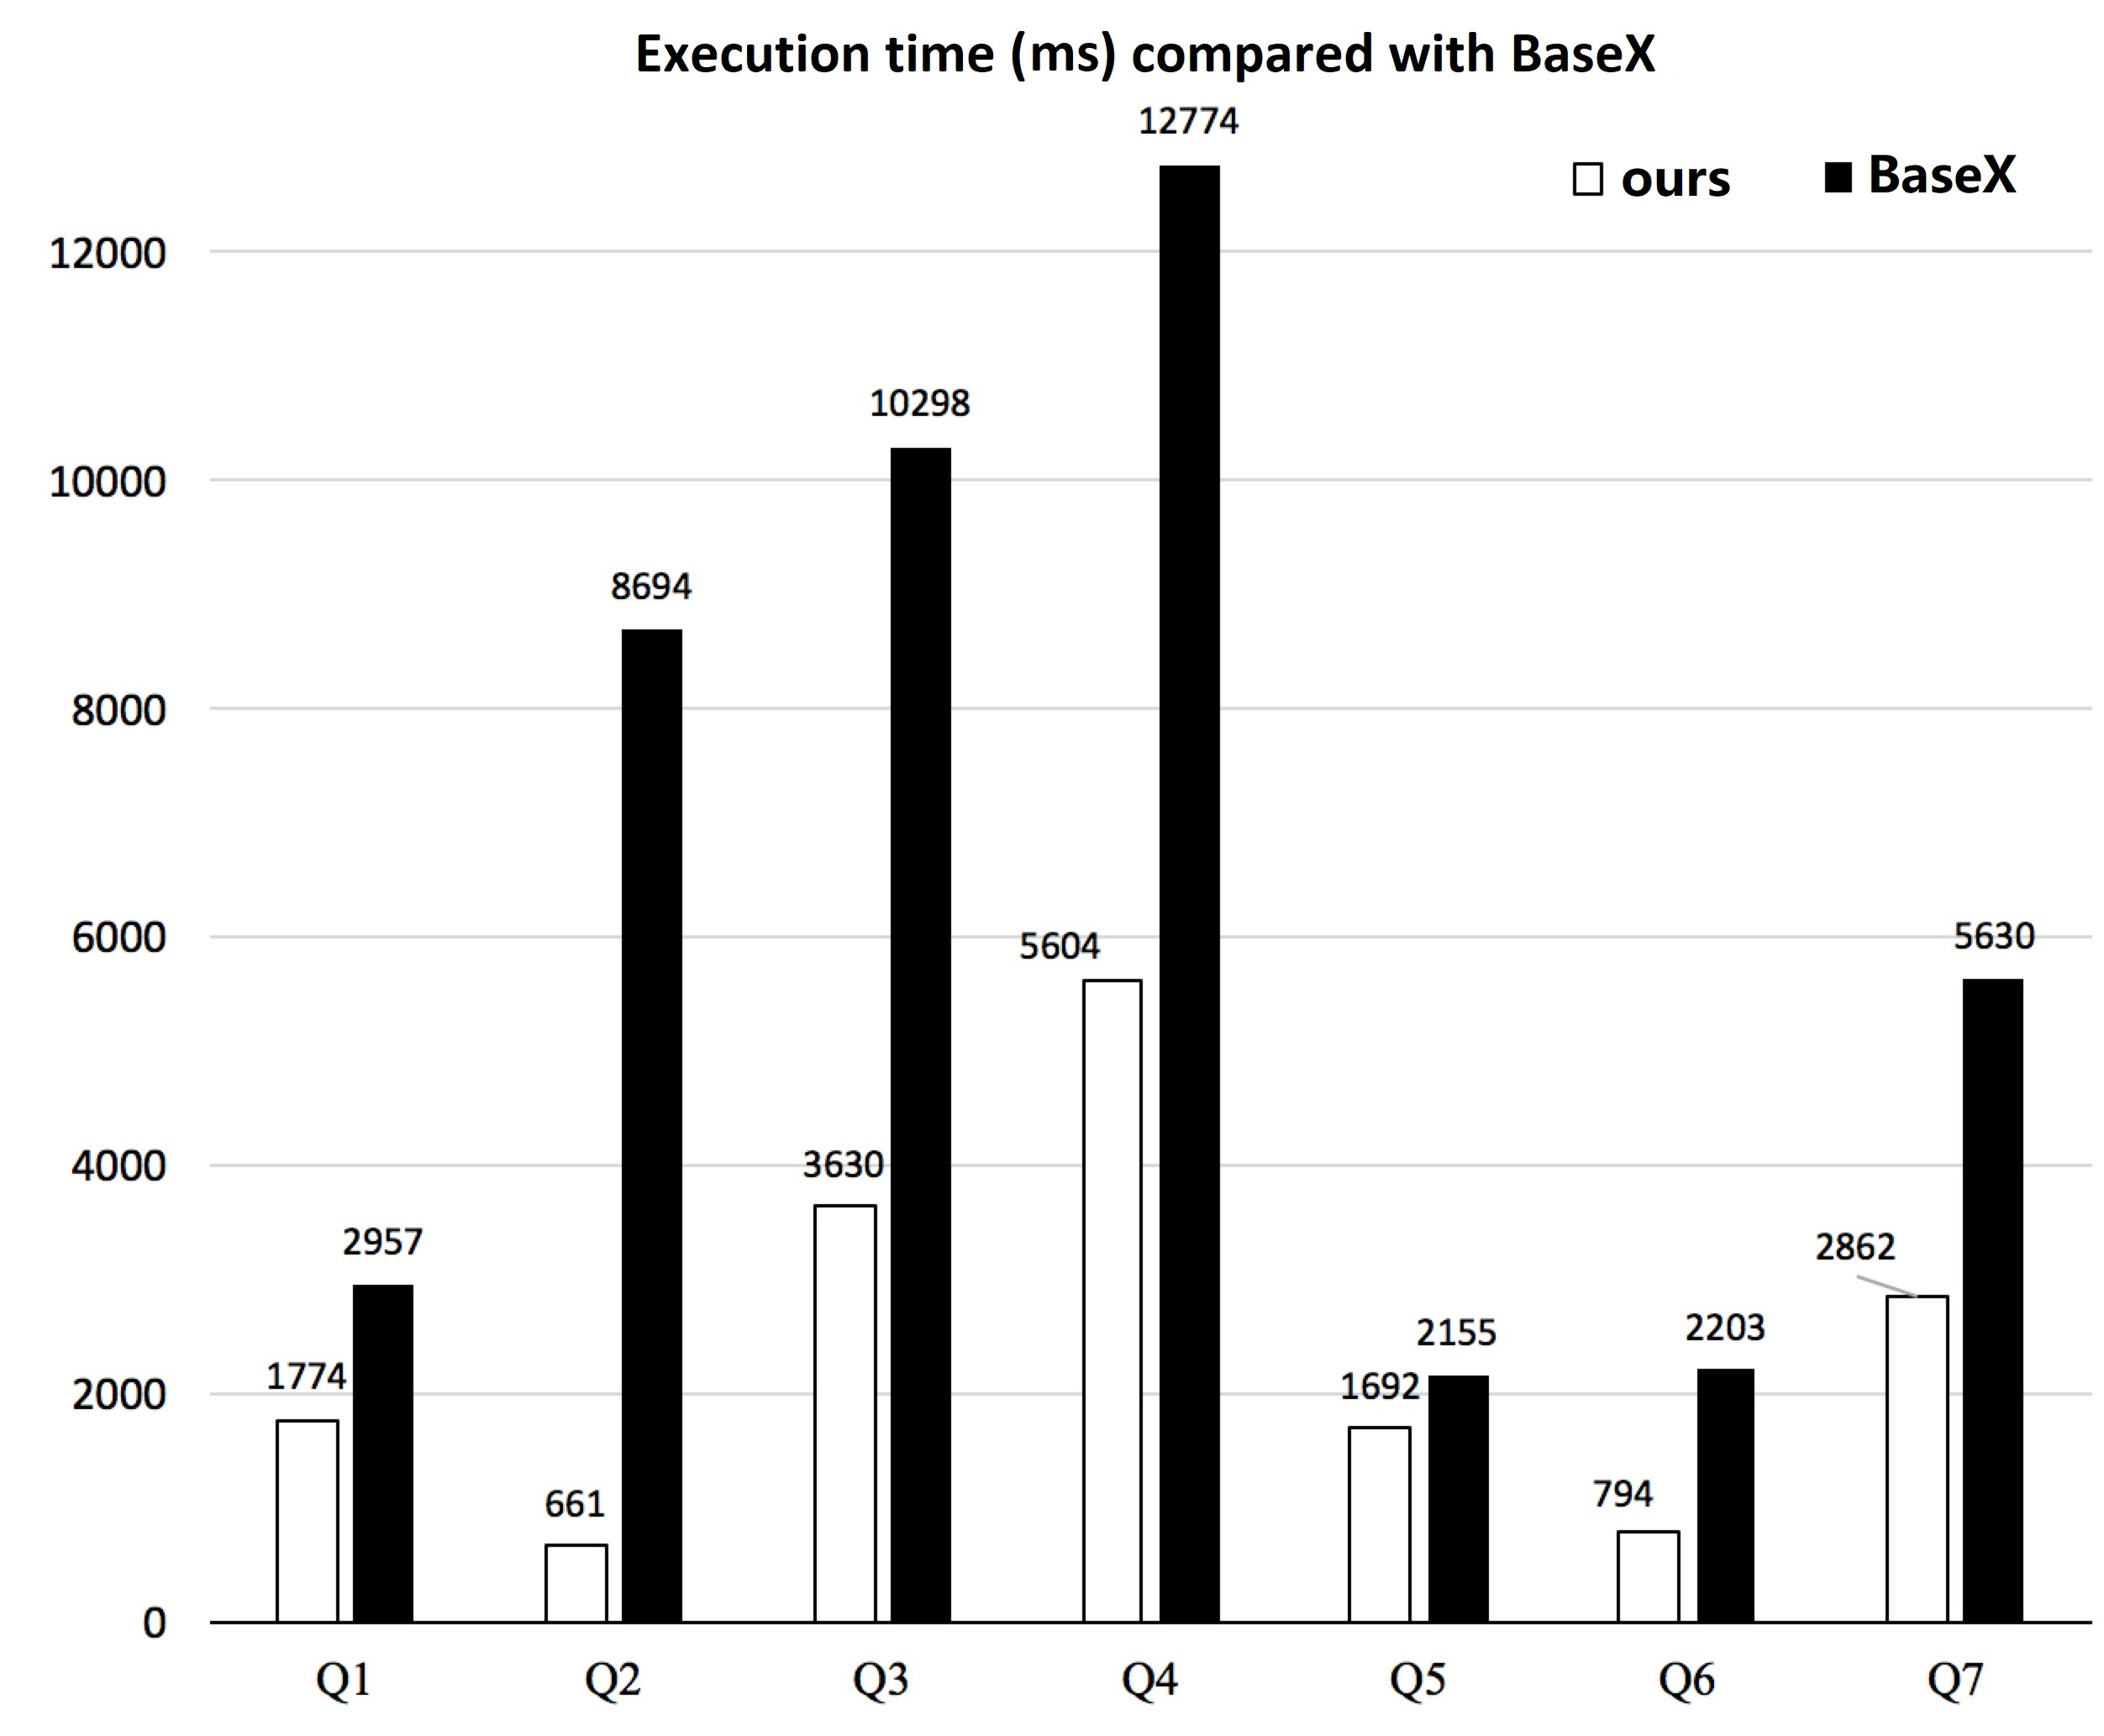
\includegraphics[width=0.9\linewidth]{compare}
	% figure caption is below the figure
	\label{fig:compare}       % Give a unique label
	\caption{Execution time (ms) compared with BaseX.}
\end{figure}

\begin{figure}[thb]
	\centering
	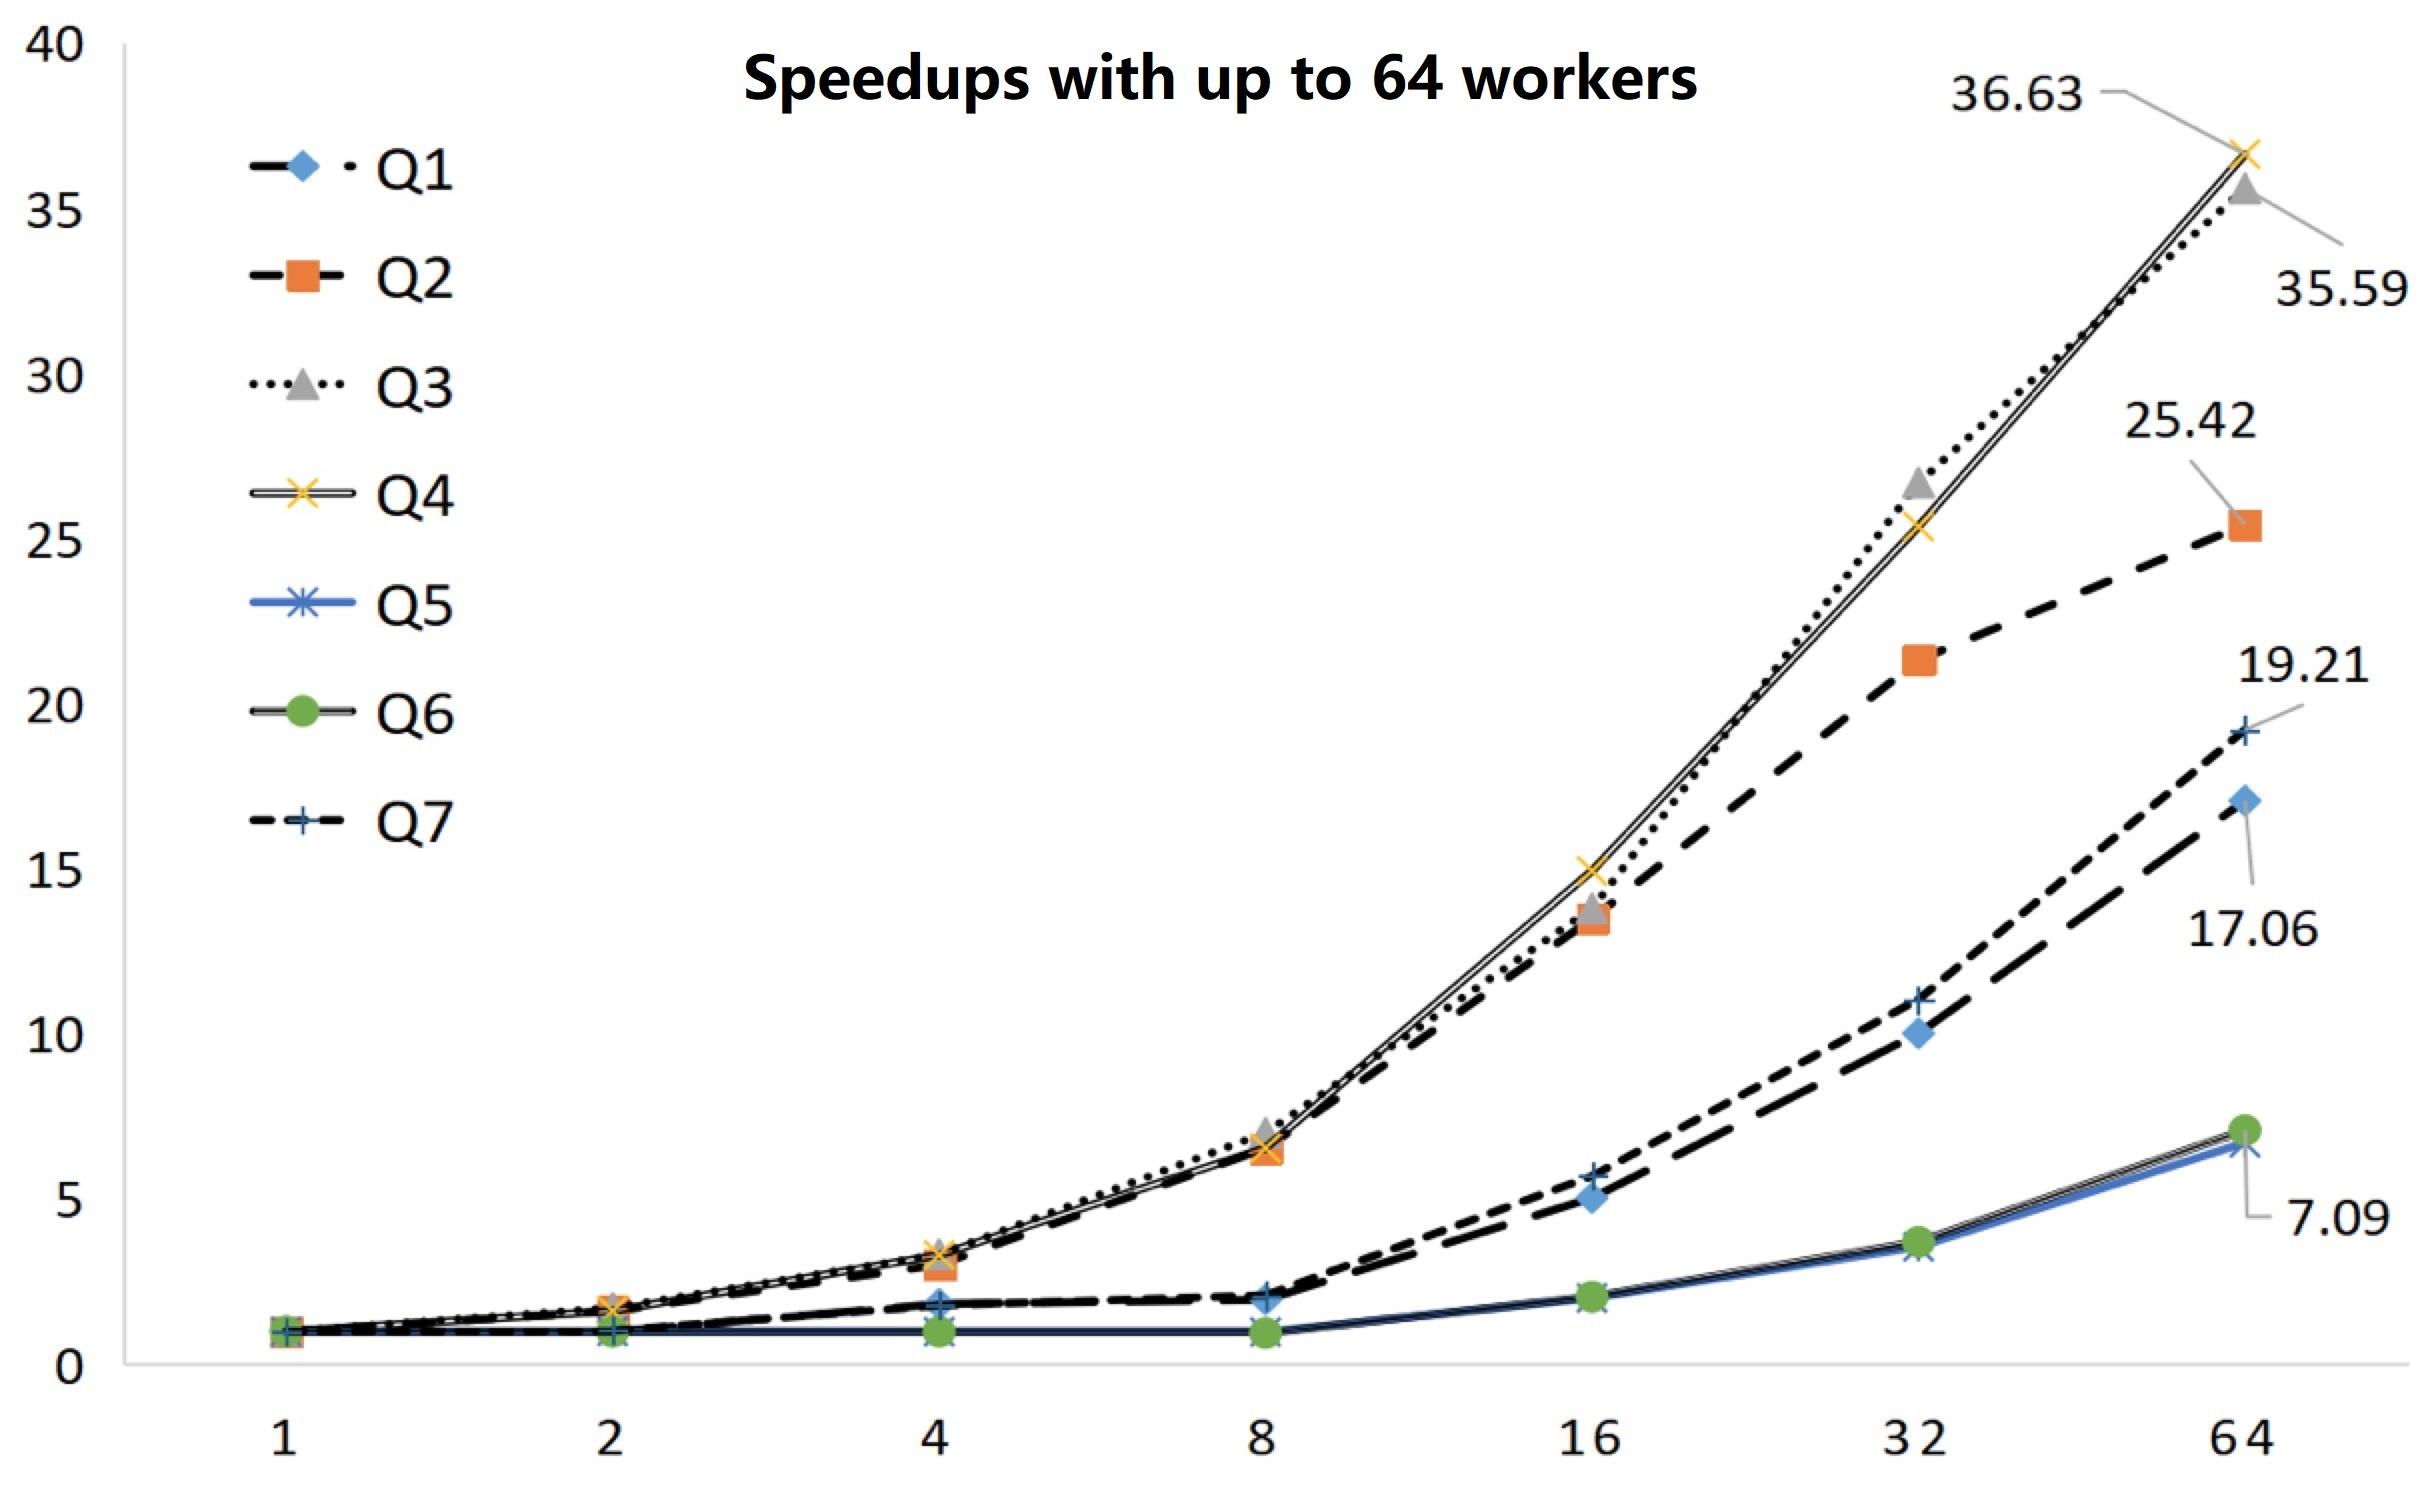
\includegraphics[width=0.9\linewidth]{speedups}
	\caption{Speedups with up to 64 workers.}
	\label{fig:speedups}    
\end{figure}


\subsubsection{Processing Queries in Parallel With Mutiple Workers}

This experiment is to test the speedups using our indexing on multiple EC2
instances. In this experiment, we use 1 instance for the master to control
query processing and 8 instances for workers to execute queries. Since the
instance m5.2xlarge has 8 cores, we arranged at most 8 workers on a single
instance. Given 8 instances, there are totally 64 workers involved in the
computation, as well as 64 chunks we divided at most. Due to the imbalance of
xmark160, not all the worker may have hit nodes of running queries. Thus, we
call workers that have hit nodes active workers, while for the rest idle
worker. 

The XML dataset xmark160 is divided into different number of chunks, to be
processed by different numbers of workers on up to 8 instances. From each chunk,
a partial tree will be created. It will be possessed and processed by a single
worker (we assign only one chunk to a worker in this experiment). 

To achieve better load balance, we used cyclic distribution to assign chunks to
instances. This means that we assign chunks to each instance, making consecutive
chunks be assigned to different instances. For example, given 8 chunks, $chunk_1$,
$chunk_2$, ..., $chunk_9$,  and 4 computing nodes, $com_1$, $com_2$, ..., $com_4$, 
we assign them as 
$com_1$($chunk_1$, $chunk_5$), 
$com_2$($chunk_2$, $chunk_6$), 
$com_3$($chunk_3$, $chunk_7$), 
$com_4$($chunk_4$, $chunk_8$). 
In such order, we can make the workers utilize the resources of computing nodes. 

We record the wall-clock time form the master's side. The timing starts from the
master sending a message to all workers to start a query, and ends at the moment
when the master receives the work-done message from the last worker, denoting
querying work is complete. The execution times are listed in
Table~\ref{tab:exetimes}.


\begin{table*}[ht]
	\centering
	\caption{Execution time in milliseconds).}
	\label{tab:exetimes}
	\begin{tabular}{|c|c|c|c|c|c|c|c|}
		\hline
		\# of workers & 1       & 2       & 4       & 8       & 16      & 32      & 64      \\ \hline
		Q1                & 1774    & 1789    & 968     & 905     & 352     & 177     & 104 \\ \hline
		Q2                & 661     & 410     & 219     & 101     &  49     & 31      & 26 \\ \hline
		Q3                & 3630    & 2120    & 1090    & 518     & 263     & 136     & 102 \\ \hline
		Q4                & 5604    & 3467    & 1695    & 855     & 375     & 221     & 153 \\ \hline
		Q5                & 1692    & 1685    & 1709    & 1731    & 841     & 475     & 252 \\ \hline
		Q6                & 794     & 800     & 803     & 834     & 388     & 214     & 112 \\ \hline
		Q7                & 2862    & 2817    & 1595    & 1369    & 502     & 259     & 149 \\ \hline
	\end{tabular}
\end{table*}

From the results, we have the following observations.

\subsubsection{Execution Time Reduced with More Workers}

From the results in the table, it is clear that with the number of workers
increased, the execution times of most queries are reduced. For
example, the execution time is nearly halves every time when the number of
workers doubled for Q3. It clearly showed that the parallel processing of
XPath queries using our index is efficient to reduce execution time by using 
more workers.

\subsubsection{Imbalance of XML Document Can Prevent Speedups}

As we can also notice, however, there are some cases execution times do not
reduce at all even with more workers. For example, no matter the number of
workers increased is 1, 2, 8 or 8, the execution times of all the cases are
still basically the same.  We analyzed the number of active workers and found
that this is caused by the imbalance of XMark datasets. In the xmark160, the hit
nodes of queries may only reside on a consecutive part of the XML document.
Then, after being divided, the hit nodes may be distributed in a small number of
chunks. Thus, only the workers that possess these chunks can be active, while
the rest workers just stay idle. Let us continue to take Q5 as an example. When
the number of workers increases from 1 to 8, the number of active nodes,
however, does not increase and still stays 1, i.e. there was only one active
worker for the query. Therefore, with only one worker, it takes nearly the same
amount of time to process the same amount of hit nodes regardless how many
workers were totally used. 

\subsubsection{Imbalance of XML Document Can Spoil Speedups}

We also notice that some execution times are not reduced much when even when
more active workers involve. For example, Q2 takes 661 ms by one active worker
and 410 ms for two active workers, the execution is not halved. This is because
the hit nodes did not evenly distributed over the two active workers. As we
investigated, one worker took 406 ms to collect 6785094 hit nodes, while another
worker took 256 ms for 4486577 hit nodes. Therefore, the speedup is degraded due
to the imbalanced distribution of hit nodes over chunks. We can learn that the
imbalance can not only prevent the speedup, but also can degrade the speedup.

To understand how much speedup ours can achieve, we use the execution time done
by a single worker as baseline. The results are shown in
Figure~\ref{fig:speedups}.  From the figure, it shows that ours can achieve
better speedup when using more workers. The best speed up is done from Q3 by a
factor of 36.63. We also notice that when the number of workers are large than
8, the speedup becomes dramatical, which means with more chunks divided, the
imbalance can be smoothed and it can be more effective for better speedups. This
is because  with smaller chunks, hit nodes can be distributed to more chunks;
meanwhile,  with the cyclic distribution of these small chunks, we can have more
active workers to participate in the querying process, thus achieving better
speedups. 


\subsubsection{Discussion}

From the experiment results and our analysis in previous sub section, we suggest
that it is better to assign more chunks to a worker rather than one as what we
conducted in the experiment. In such case, more workers will possess chunks that
contain hit nodes. In ideal case, hit nodes consecutively contained in a part of
the XML document can be divided into more chunks, and these chunks can be
distributed to each of workers.  Then, all the workers become active and we can
achieve better speedups. However, with too many chunks, it is not clear how
much overhead on memory, thread or network etc will be involved. We need to find
a trade-off about the maxamum number of chunks to reach the best performance.
Thus, it is worth studying for the future work.



